\section{Optimisation discrète}

\begin{enumerate}

  \item Considérez le problème d'optimisation en nombres entiers

    $
    \begin{array}{lrcrcl}
      \maxi & 5x_1 & +&  x_2\\
      & -x_1 &+& 2 x_2  & \leq & 4 \\
      & x_1    & - &    x_2   &  \leq & 1\\
      &   4x_1& +&  x_2  & \leq & 12 \\
      &   \multicolumn{3}{r}{x_1, x_2}  & \geq & 0\\
      &   \multicolumn{3}{r}{x_1, x_2}  & \multicolumn{2}{l}{\mbox{ entiers}}
    \end{array}
    $

    Trouvez graphiquement une solution de ce problème. Trouvez graphiquement une solution optimale du problème relaxé. Trouvez la
    solution entière la plus proche de la solution optimale du problème relaxé. Enumérez toutes le solutions entières obtenues en
    arrondissant la solution optimale du problème relaxé. Une de ces solutions est-elle optimale?


    \begin{solution}
      On voit que la solution optimale entière est $x^* = (2,3)$ qui donne
      un coût optimal de 13.
      La solution optimale du problème relaxé est $\frac{1}{5}(13,8)$.
      Les solutions admissibles obtenues en arrondissant cette solution
      sont $(2,1)$ et $(2,2)$ qui donnent respectivement un coût optimal de
      11 et 12.
      Ce ne sont donc pas des solutions optimales.
    \end{solution}

  \item Yves et Muriel désirent partager les principales tâches ménagères  (courses, cuisine, vaisselle et nettoyage)
    entre eux. Leurs efficacités à la réalisation de ces tâches
    diffèrent. Yves est rapide pour faire les courses et la vaisselle mais il se fait distancer par Murielle pour la cuisine et le
    nettoyage.

    \begin{center}
      \begin{tabular}{l|llll}
        & courses & cuisine & vaisselle & nettoyage\\
        \hline
        Yves & 4.5 & 7.8 & 3.6 & 3.1\\
        Muriel & 4.9 & 7.2 & 4.3 & 2.9
      \end{tabular}
    \end{center}

    Le jeune couple  désire partager les tâches de manière équitable (deux tâches par personne) et optimale (temps total minimum). Formulez
    ce problème comme un problème d'optimisation en nombres entiers. Donnez une relaxation de ce problème. La solution du problème
    relaxé est-elle entière? Que pouvez-vous en déduire?


    \begin{solution}
      Soient $x_{ij}$ valant 1 si $i$ fait la tâche $j$ et 0 sinon
      et $c_{ij}$ le temps que fait $i$ pour faire la tâche $j$.
      Le problème devient alors
      \begin{align*}
        \min \sum_{ij}c_{ij}x_{ij}\\
        \sum_{j} x_{ij} & = 2 && i = 1,2\\
        \sum_{i} x_{ij} & = 1 && j = 1,2,3,4\\
        x_{ij} & \in \lbrace 0,1\rbrace.
      \end{align*}
      La solution optimale du problème relaxé est
      \[ x^* =
        \begin{pmatrix}
          1 & 0 & 1 & 0\\
          0 & 1 & 0 & 1
      \end{pmatrix}. \]
      Elle est entière, elle est donc solution optimale du problème non-relaxé.

      On peut aussi le démontrer par l'absurde comme suit:
      \begin{proof}
        Soit une solution différente,
        posons $\delta > 0$ la plus petite variation non
        nulle d'une variable de la solution à la solution $x^*$.
        Sans perte de généralité, disons que c'est à la variable $x_{23}$.
        On a donc $x_{13} \leq 1 - \delta$. Il y a donc soit $x_{12}$,
        soit $x_{14}$ qui est non-nulle et comme on a supposé $\delta$ comme
        étant la plus petite variation,
        au moins un des deux a une variation plus grande que $\delta$.
        Sans perte de généralité, disons que c'est $x_{12}$.
        Enretirant $\delta$ à $x_{13}$ et $x_{22}$
        et en ajoutant $\delta$ à $x_{23}$ et $x_{12}$,
        on a donc toujours une solution admissible donc le coût
        change de $\delta(4.3-3.6 +7.8-7.2) > 0$ et donc augmente.
        La solution n'est donc pas optimale d'où la contradiction.
      \end{proof}
      On remarque que la solution du problème relaxé est entière.
      Elle est donc aussi solution optimale du problème non relaxé.
    \end{solution}

  \item Vouz désirez choisir un ensemble de cours parmi huit cours $\{1, \ldots,
    8 \}$ pour vous constituer un programme. Modélisez les contraintes
    suivantes:

    \begin{enumerate}
      \item Vous ne pouvez pas choisir plus de 5 cours mais devez en choisir au
        moins 3.
      \item Le cours 3 est un prérequis du cours 6 et le cours 2 un prérequis
        du cours 7.
      \item Les cours 8 et 6 forment une paire. Vous devez les prendre tous les
        deux, ou aucun des deux.
      \item Pour des questions de conflit horaire, vous ne pouvez pas choisir
        les cours 5 et 2, ni les cours 3 et 6.
      \item Pour vous conformer aux contraintes de votre programme d'étude vous devez choisir au moins un des cours
        1, 2, 3 ou au moins deux cours parmi les cours 5, 6, 7, 8.
    \end{enumerate}


    \begin{solution}
      Soit $x_i$ valant 1 si le cours $i$ est choisi et 0 sinon.
      \begin{enumerate}
        \item $3 \le \sum_{i} x_{i} \le 5$.
        \item $x_{6} \le x_{3}$ et $x_{7} \le x_{2}$.
        \item $x_{6} = x_{8}$.
        \item $x_{2} + x_{5} \le 1$ et $x_{3} + x_{6} \le 1$.
          $x_2x_5 = 0$ n'est pas correct car ce n'est pas linéaire.
        \item $ 1-y \le x_{1} + x_{2} + x_{3}$ et
          $ 2y \le x_{5} + x_{6} + x_{7} + x_{8}$
          où $y \in \lbrace 0,1\rbrace$.
      \end{enumerate}
    \end{solution}

  \item Vous désirez trouver les variables $0 \leq x_1, x_2 \leq 1$ qui maximisent la fonction $c^T x$ tout en satisfaisant au
    moins une  des deux contraintes $x_1 + 2 x_2 \leq 1$  et  $3 x_1 +  x_2 \leq 1$. Formulez ce problème comme un
    problème d'optimisation mixte.

    \begin{solution}
      Comme $x_1,x_2 \leq 1$, si on transforme les conditions en
      $x_1 + 2x_2 \leq 3$ et $3x_1 + x_2 \leq 4$,
      on ne contraint plus rien du tout.
      On peut donc modéliser le problème comme suit
      \begin{align*}
        x_1 + 2x_2 & \leq 1 + 2b_1\\
        3x_1 + x_2 & \leq 1 + 3b_2\\
        b_1 + b_2 & \leq 1\\
        (x,b) & \leq 1\\
        (x,b) & \geq 0\\
        b & \text{ entiers}
      \end{align*}
      où les $b_i$ ne peuvent être nuls que si leur contrainte respective
      est respectée sans leur aide (e.g. $x_1 + 2x_2 \leq 1$).
      C'est aussi correcte de prendre le problème suivant
      \begin{align*}
        x_1 + 2x_2 & \leq 1 + 2b\\
        3x_1 + x_2 & \leq 1 + 3(1-b)\\
        (x,b) & \leq 1\\
        (x,b) & \geq 0\\
        b & \text{ entiers}.
      \end{align*}
    \end{solution}

  \item Une société a développé deux nouveaux jouets pour la Noël. La production du jouet 1 nécessite des investissements initiaux de
    50000 EUR et celle du jouet 2 des investissements initiaux de 80000 EUR. Les jouets
    génèrent un profit de 10 EUR pour le jouet 1 et de 15 EUR pour le jouet 2.  Le jouet 1 est
    produit à un taux de 50 l'heure et le jouet 2 à un taux de 25 l'heure. On dispose  de 500 heures
    d'ici Noël. Déterminez le nombre de jouets à produire de manière à maximiser le profit.


    Supposons maintenant que la société possède deux usines. Une seule usine sera choisie pour la production. Le
    jouet 1 est produit à un taux de 50 l'heure dans l'usine 1 et de 40 l'heure dans l'usine 2. Le jouet 2 est produit à un taux de
    25 l'heure dans les deux usines. Les usines disposent de 500 et 700 heures d'ici Noël.  Le problème consiste à déterminer le
    nombre de jouets à produire de manière à maximiser le profit.

    \begin{solution}
      \nosolution
    \end{solution}

  \item Vous disposez de 4 objets de poids respectifs 5, 3, 8 et 7. Les utilités des
    objets sont de 17, 10, 25 et 7. Vous désirez sélectionner un ensemble d'objets de poids total inférieur  à 12 et dont la somme
    des utilités est maximale.  Formulez le problème comme un problème d'optimisation en nombres entiers. Trouvez la solution.


    \begin{solution}
      Le problème d'optimisation est le suivant
      \begin{align*}
        \max 17x_1 + 10x_2 + 25x_3 + 7x_4\\
        5x_1 + 3x_2 + 8x_3 + 7x_4 & \leq 12\\
        x & \in \{0,1\}
      \end{align*}
      où $x_i$ vaut 1 si on prend l'objet et 0 sinon.
      
      La solution optimale du problème relaxé est $(1,1,0.5,0), qui n'est pas entière.
      Celle-ci donne une utilité de 39.5.
      Comme le problème est petit, on peut le résoudre en nombres entiers facilement à la main.
      En effet, on peut essayer de combiner différents objets en connaissant le rapport utilité/poids
      (qui est ici $(17/5,10/3,25/8,1)$). 
      Si on prend le premier, qui a le meilleur rapport, on peut encore prendre le deuxième.
      En prenant le deuxième et le troisième, on a une plus grande utilité.
      En essayant d'autres combinaisons, on voit qu'il s'agit de la solution optimale en nombres entiers.
      Heureusement, la solution du problème non est donc $(0,1,1,0)$.
    \end{solution}

  \item Vous disposez de 5 objets de poids respectifs 2, 4, 3, 3 et 2. Les
    utilités des objets sont respectivement de 9, 20, 14, 10 et 6. Vous désirez
    sélectionner un ensemble d'objets de poids total inférieur  à 10
    et dont la somme des utilités est maximale.  Formulez le problème
    comme un problème d'optimisation en nombres entiers. Appliquez l'algorithme ``branch and bound'' pour trouver la
    solution. Justifiez les étapes de l'algorithme.

    \begin{solution}
      Le problème d'optimisation est le suivant
      \begin{align*}
        \max 9x_1 + 20x_2 + 14x_3 + 10x_4 + 6x_5 & \leq 10\\
        2x_1 + 4x_2 + 3x_3 + 3x_4 + 2x_5 & \leq 10\\
        x & \in \{0,1\}
      \end{align*}
      où $x_i$ vaut 1 si on prend l'objet et 0 sinon.

      Pour résoudre la relaxation, il suffit d'augmenter $x_i$ où tel que
      $c_i/a_i \geq c_j / a_j$ pour tout $j$ tel que $x_j < 1$.
      Quand $x_i$ arrive à 1, on en sélectionne un autre et ainsi de suite
      jusqu'à ce que $a^Tx = 10$.
      Ici, les $c_i/a_i$ valent
      \[ \begin{pmatrix}
          \frac{9}{2} & 5 & \frac{14}{3}
          & \frac{10}{3} & 3
        \end{pmatrix}
      \]
      On les prend donc dans l'ordre $2, 3, 1, 4, 5$.

      L'algorithme de branch and bound nous donne alors

      \Tree [.{$(1,1,1,1/3,0) \rightarrow 46.\bar{3}$}
        [.{$x_4 \leq 0$\\$(1,1,1,0,1/2) \rightarrow 46$}
          [.{$x_5 \leq 0$\\$(1,1,1,0,0) \rightarrow 43$} ]
          [.{$x_5 \geq 1$\\$(1/2,1,1,0,1) \rightarrow 44.5$} ]
        ]
        [.{$x_4 \geq 1$\\$(0,1,1,1,0) \rightarrow 44$} ]
      ]

      On sait qu'en continuant, on ne fera pas mieux que 44 car
      on sera $\leq 44.5$ et entier car les $c_i$ sont entiers.
      On trouvera par contre peut-être d'autres solutions optimales
      (ici, ce n'est pas le cas),
      mais si une solution optimal nous suffit,
      ça ne sert à rien de continuer.
      La solution optimale est donc $x^*=(0,1,1,1,0)$ avec comme
      coût optimal $z^*=44$.
    \end{solution}

  \item  Considérez l'arbre d'énumération suivant pour un problème
    d'optimisation en nombres entiers.
    L'arbre résulte-t-il d'un problème de maximisation ou de minimisation?
    Quels sont les noeuds qui doivent encore être analysés?
    Donnez un intervalle dans lequel se trouve l'optimum.
    Que pouvez vous dire de la solution optimale?
    % FIXME quel arbre ?

    \begin{solution}
      \nosolution
    \end{solution}

  \item Considérez le problème d'optimisation en nombres entiers

    $
    \begin{array}{lrcrcl}
      \maxi & 9x_1 & +&  5 x_2\\
      & 4 x_1 &+& 9 x_2  & \leq & 35 \\
      & x_1    &  &       &  \leq & 6\\
      &   x_1& -&  3x_2  & \geq & 1 \\
      & 3 x_1    & + & 2x_2   &  \leq & 19\\
      &   \multicolumn{3}{r}{x_1, x_2}  & \multicolumn{2}{l}{\mbox{ entiers}}
    \end{array}
    $


    Résolvez le problème graphiquement et algébriquement
    en utilisant la méthode ``branch and bound''.

    \begin{solution}
      Le problème peut être illustré par le graphique suivant qui va nous être
      utile dans la méthode ``branch and bound''.
      \begin{center}
        \begin{tikzpicture}
          % Axis
          \draw[axis] (0,0) -- (6.5,0) node[right=\nudge cm] {\(x_1\)};
          \draw[axis] (0,0) -- (0,2) node[above=\nudge cm] {\(x_2\)};
          \begin{scope}
            % Avoid going too far
            \clip (-\nudge,-\nudge) rectangle (6.5+\nudge,2+\nudge);
            \draw[line] (35/4,0) -- (3,23/9) coordinate (ineq1);
            \draw[line] (6,-1) -- (6,3) coordinate (ineq2);
            \draw[line] (0,-1/3) -- (7,2) coordinate (ineq3);
            \draw[line] (19/3,0) -- (4.5,5.5/2) coordinate (ineq4);
            \draw[obj] (56.5/9,0) -- (4.5,3.2);
            \begin{scope}
              %Clip sélectionne ce qu'il y a dans le polygone dessiné.
              \clip (1,0) -- (59/11,16/11) -- (6,1/2) -- (6,0);
              \fill[hash] (0,0) rectangle (6,2);
              %\draw[dashed,line] (0,1) -- (2,2) -- (3,1) -- (2,0);
              % (4,4) to be enough, anyway clip restrict us to the good part
            \end{scope}
          \end{scope}
          \node[left] at (ineq1) {\(4x_1 + 9 x_2 = 35\)};
          %\node[right] at (ineq1) {\(\mathllap{-}y_1 + y_2 = 3\)};
          %\node[right] at (ineq2) {\(\mathllap{-}y_1 - y_2 = -1\)};
          \node[right] at (ineq3) {\(x_1 - 3x_2 = 1\)};
          \node[above] at (ineq4) {\(3x_1 + 2x_2 = 19\)};
          \foreach \coord/\adj in {
            {(1,0)}/below,
            {(6,0)}/below right,
            {(59/11,16/11)}/left,
            {(6,1/2)}/right%
          } {
            \fill \coord circle (2pt) node[\adj] {$\coord$};
          }
          \foreach \coord in {
                                       {(4,1)}, {(5,1)},
            {(1,0)}, {(2,0)}, {(3,0)}, {(4,0)}, {(5,0)}, {(6,0)}
          } {
            \fill[intdom] \coord circle (1.5pt);
          }
        \end{tikzpicture}
      \end{center}
      La méthode ``branch and bound'' nous donne

      \Tree [.{$(6,1/2) \rightarrow 56.5$}
        [.{$x_2 \leq 0$\\$(6,0) \rightarrow 54$} ]
        [.{$x_2 \geq 1$\\$(17/3,1) \rightarrow 56$}
          [.{$x_1 \leq 5$\\$(5,4/3) \rightarrow 51.\bar{6}$} ]
          [.{$x_1 \geq 6$\\$\mathcal{D}=\emptyset$} ]
        ]
      ]

      où la solution $x^*=(6,0)$ apparait clairement avec $z^* = 54$.
    \end{solution}

  \item Considérez l'arbre d'énumération suivant pour un
    problème d'optimisation de deux variables entières
    où ``E'' signifie que la solution optimale du problème
    relaxée est entière et ``NE'' signifie qu'elle n'est pas entière.

    \Tree [.{60 NE}
      [.{59.8 NE}
        [.{50.2 NE} ]
        [.{48 E} ]
      ]
      [.{56.7 NE}
        [.{51 E} ]
        [.{53.4 NE} ]
      ]
    ]

    \begin{enumerate}
      \item L'arbre résulte-t-il d'un problème de maximisation ou de minimisation?
      \item \label{r1} Quels sont les
        noeuds qui doivent encore être analysés?
      \item \label{r2} Donnez un intervalle dans lequel se trouve
        l'optimum.
      \item La fonction objectif est donnée
        par $3x_1+6x_2$. Cette information vous permet-elle de préciser vos réponses aux sous-questions \ref{r1} et
        \ref{r2}?
    \end{enumerate}

    \begin{solution}
      \begin{enumerate}
        \item C'est un problème de maximisation car 60 est la solution
          du problème complet alors que 59.8 est celle
          d'une restriction et que $59.8 < 60$.
        \item 50.2 ne doit pas être exploré car il est plus petit que 51.
          53.4 doit par contre être exploré.
        \item On sait que $51 \leq z^* \leq 53.4$.
        \item On sait alors que si $x_1$ et $x_2$ sont entiers,
          $z^*$ sera divisible par 3.
          Comme le prochain multiple de 3 après 51 est 54,
          on sait que $z^* = 51$ et il ne vaut plus explorer 53.4.
      \end{enumerate}
    \end{solution}

  \item  Il y a 50 groupes d'étudiants en première candidature FSA. On souhaite affecter un projet par groupe. Il y a 10
    projets disponibles et chaque projet peut être affecté à au plus 10 groupes. On a demandé à chaque groupe de classer les trois projets qui ont leur
    préférence. On souhaite affecter à chaque groupe un des projets qu'il a classés et maximiser le nombre de groupes qui recoivent leur premier choix.
    S'il y a plusieurs affectations qui satisfont cette contrainte, on souhaite, parmi l'ensemble de ces affectations, choisir celle qui maximise le nombre de groupes
    qui recoivent leur deuxième choix. Vous êtes coordinateur d'année en FSA; proposez une manière de résoudre ce problème.


    \begin{solution}
      \nosolution
    \end{solution}

  \item Le Sudoku est un jeu logique présenté sous forme de grille.
    D'abord publié en 1979, le Sudoku s'est développé au Japon en 1986 avant d'atteindre la popularité internationale en 2005, et ce jusqu'aux colonnes de l'hebdomadaire ``la Salopette'' édité par le CI.
    La grille de jeu est un carré de neuf cases de côté, subdivisé en neuf carrés, appelés régions (voir figure).
    Quelques chiffres sont disposés dans la grille et le but du jeu est de compléter la grille avec des chiffres  de un à neuf en respectant la règle suivante: chaque ligne, colonne et région ne doit contenir qu'une et une seule fois  les chiffres de un à neuf.

    \begin{enumerate}

      \item Formulez le problème du Sudoku pour une grille quelconque comme
        un problème  d'optimisation linéaire en nombres entiers.

      \item Une grille de Sudoku peut ne pas avoir de solution.
        Si une grille ne possède pas de solution,
        un objectif naturel consiste
        à compléter  toutes les cases de manière à ce que
        le nombre total de lignes,
        colonnes et régions complètes soit aussi élevé que possible
        (une ligne, colonne ou région est complète si tous les nombres de
        un à neuf y apparaissent exactement une fois).
        Formulez ce problème comme un problème d'optimisation linéaire
  en nombres entiers.

        \begin{center}
          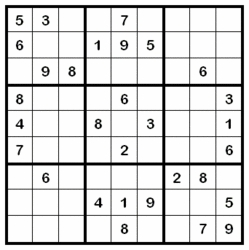
\includegraphics[scale=0.7]{sudo.jpg}
        \end{center}

    \end{enumerate}

    \begin{solution}
      Soient
      \[ x_{ijk} =
        \begin{cases}
          1 & \text{si la case }i, j\text{ a la valeur }k\\
          0 & \text{sinon}
        \end{cases}
      \]
      et $I = \{1,2,\ldots,9\}$
      \begin{enumerate}
        \item Le problème d'optimisation linéaire est le suivant
          \begin{align*}
            \min 1\\
            \sum_{j=1}^9 x_{ijk} & = 1 & \forall i,k \in I\\
            \sum_{i=1}^9 x_{ijk} & = 1 & \forall j,k \in I\\
            \sum_{i=r}^{r+2}\sum_{j=c}^{c+2} x_{ijk} & = 1
            & \forall r \in \{1,4,7\}, c \in \{1,4,7\}\\
            \sum_{k=1}^9 x_{ijk} & = 1 & \forall i,j \in I\\
            x & \leq 1\\
            x & \geq 0\\
            x & \text{ entiers}.
          \end{align*}
          La première (resp. deuxième) condition s'assure qu'on a bien complété
          les lignes (resp. les colonnes).
          La troisième fait de même pour les régions.
          La quatrième s'assure qu'on a complété un seul chiffre par
          case.
          Les 3 dernières s'assurent que $x$ contient des variables binaires.
        \item
          On va poser
          \begin{itemize}
            \item $a_i$ valant 1 si la ligne $i$ est complétée correctement
              et 0 sinon;
            \item $b_j$ valant 1 si la colonne $j$ est complétée correctement
              et 0 sinon;
            \item $c_{ij}$ valant 1 si la région donc un coin est en
              $(i,j)$ est complétée correctement
              et 0 sinon.
          \end{itemize}
          On peut alors exprimé le problème en le problème d'optimisation
          linéaire suivant
          \begin{align*}
            \max \sum_{i=1}^9 a_i + \sum_{j=1}^9 b_j +
            \sum_{r\in\{1,4,7\}}\sum_{c\in\{1,4,7\}} c_{rc}\\
            \sum_{j=1}^9 x_{ijk} & \leq 1 & \forall i,k \in I\\
            \sum_{i=1}^9 x_{ijk} & \leq 1 & \forall j,k \in I\\
            \sum_{i=r}^{r+2}\sum_{j=c}^{c+2} x_{ijk} & \leq 1
            & \forall r \in \{1,4,7\}, c \in \{1,4,7\}\\
            \sum_{k=1}^9 x_{ijk} & \leq 1 & \forall i,j \in I\\
            \sum_{k=1}^9\sum_{j=1}^9 x_{ijk}
            & \geq 9a_i & \forall i \in I\\
            \sum_{k=1}^9\sum_{i=1}^9 x_{ijk}
            & \geq 9b_j & \forall j \in I\\
            \sum_{k=1}^9\sum_{i=r}^{r+2}\sum_{j=c}^{c+2} x_{ijk}
            & \geq 9c_{rc}
            & \forall r \in \{1,4,7\}, c \in \{1,4,7\}\\
            (x,a,b,c) & \leq 1\\
            (x,a,b,c) & \geq 0\\
            (x,a,b,c) & \text{ entiers}.
          \end{align*}
      \end{enumerate}
    \end{solution}

  \item \textsc{OptiTv} lance un nouveau jeu sur nos écrans.  La
    dernière épreuve du jeu permet au gagnant de
    multiplier ses gains.

    Deux rails $A$ et $B$ traversent un plateau de jeu jonché
    d'obstacles.  Le but du joueur est de maximiser la masse
    totale
    de deux billes posées sur les rails qui pourront traverser le plateau.
    Pour ce faire, il peut décider de retirer
    certains obstacles du parcours, mais pour chaque obstacle
    enlevé, une pénalisation de $20$ grammes lui sera retranchée du résultat.
    Les règles du jeu sont les suivantes:
    \begin{enumerate}
      \item Le joueur a à sa disposition des billes de $10$,
        $20$, $30$, ..., $100$ grammes en quantité suffisante.  Il
        peut déposer $0$, $1$ ou $2$ billes sur le plateau
        (maximum une bille par rail), et chaque bille déposée doit
        traverser de part en part le plateau sous peine de
        disqualification.
      \item Pour assurer l'équilibre du plateau, la différence
        de masse entre les deux billes choisies ne peut pas excéder
        $20$ grammes. En particulier, si une seule bille traverse le
        plateau, sa masse ne peut pas être supérieure à $20$
        grammes.
      \item Si l'obstacle $1$ n'est pas ôté,
        une bille posée sur le rail $A$ ne
        peut pas traverser le plateau de jeu.
      \item Les obstacles $2$ et $3$ ne peuvent pas être retirés
        tous les deux ensemble.
      \item S'il souhaite retirer l'obstacle $2$ ou l'obstacle
        $4$, le joueur est obligé d'enlever d'abord les obstacles
        $1$ et $3$.
%        {\it \item Le joueur est obligé d'enlever au moins un des
%        obstacles parmi $2$ et $4$ ou d'enlever les deux obstacles
%        $1$ et $3$.}
      \item Les obstacles $3$ et $4$ déterminent conjointement
        la masse maximale de la bille qui pourra passer sur le rail $B$: le
        retrait de l'obstacle $3$ permet de faire passer $80$
        grammes et le retrait de l'obstacle $4$ autorise quant à lui $20$
        grammes.  En particulier, si ces deux obstacles sont
        retirés, une bille de $100$ grammes peut passer sur ce
        rail.
        %Quatre obstacles peuvent gêner la progression des billes.
    \end{enumerate}

    Formulez ce problème comme un problème d'optimisation linéaire
    en nombres entiers.  Vous ne devez pas résoudre ce
    problème.




    \begin{solution}
      \nosolution
    \end{solution}

  \item Vous disposez d'une somme de 96 Euros. Vous désirez acheter
    des boissons, disponibles en divers conditionnements.
    \begin{center}
      \begin{tabular}{|c|c|c|c|c|c|}
        \hline %\vspace{2pt}
        Boisson & A & B & C & D & E\\
        \hline
        Volume unitaire (litres) & 15 & 16 & 17 & 18 & 20\\
        \hline
        Prix unitaire (Euros) & 16 & 17 & 18 & 19 & 20\\
%\hline Nombre disponible & $\infty$ & $\infty$ & 6  & 4\\
        \hline
      \end{tabular}
    \end{center}
    Vous désirez acheter un volume le plus grand possible, sans
    dépasser votre budget.
    \begin{enumerate}
      \item Formulez ce problème comme un problème d'optimisation
        linéaire en nombres entiers.
      \item Combien de conditionnements de chaque type allez-vous acheter
        ? Détaillez votre raisonnement.
    \end{enumerate}

    \begin{solution}
      Soit $x_i$ le nombre de conditionnement $i$.
      Le problème d'optimisation est le suivant
      \begin{align*}
        \max 15x_A + 16x_B + 17x_C + 18x_D + 20x_E\\
        16x_A + 17x_B + 18x_C + 19x_D + 20x_E & \leq 96\\
        x_A,x_B,x_C,x_D,x_E & \geq 0\\
        x_A,x_B,x_C,x_D,x_E & \text{ entiers}.
      \end{align*}
      Pour le problème relaxé,
      il faut commencer par prendre les conditionnements ayant
      le meilleur ratio volume/prix.
      On doit donc les prendre dans l'ordre E, D, C, B, A.
      La méthode ``branch and bound'' nous donne

      \Tree [.{$(0,0,0,0,24/5) \rightarrow 96$}
        [.{$x_5 \leq 4$\\$(0,0,0,16/19,4) \rightarrow 95.16$}
        ]
        [.{$x_5 \geq 5$\\$\mathcal{D}=\emptyset$} ]
      ]

      où on pourrait continuer avec $x_4 \leq 0$ et $x_4 \geq 1$
      mais en remarquant que $x=(1,0,0,0,4)$ est solution admissible
      avec $z=95$, on découvre que $95 \leq z^* \leq 95.16$.
      Comme les $c_i$ sont entiers, on sait que $z^*$ est entier.
      On peut donc affirmer que $z^* = 95$ et que $x^*=(1,0,0,0,4)$ est
      une solution optimale.
    \end{solution}

  \item Un transporteur est confronté au problème suivant : il ne
    peut transporter qu'une tonne de marchandises dans son véhicule,
    alors qu'une quantité supérieure à une tonne est disponible. Il
    reçoit les données suivantes de la part du comptable de
    l'entreprise, regroupant les quantités disponibles de chaque
    marchandise, ainsi que le bénéfice retiré par leurs ventes
    respectives.

    \begin{center}
      \begin{tabular}{|c|c|c|c|}
        \hline %\vspace{2pt}
        Marchandise & A & B & C\\
        \hline
        Quantité disponible (kg) & 900 & 240 & 560 \\
        \hline
        Bénéfice (euros/kg) & 15 & 17,5 & 14 \\
        \hline
      \end{tabular}
    \end{center}

    \begin{enumerate}
      \item D'après ces informations, formulez le problème d'optimisation
        linéaire correspondant et déterminez les quantités de A,B et C qui
        optimiseront le bénéfice réalisé par la vente du chargement et
        donnez la valeur de ce bénéfice.

        \vspace{6pt} Arrivé dans le hangar pour charger, le chauffeur
        réalise que les marchandises sont conditionnées en sacs, et qu'il
        est impensable de charger autres choses que des sacs complets.
        Voici les poids des sacs qui constituent le stock :
        \begin{center}
          \begin{tabular}{|c|c|c|c|}
            \hline %\vspace{2pt}
            Marchandise & A & B & C\\
            \hline
            Poids d'un sac (kg) & 60 & 80 & 20 \\
            \hline
          \end{tabular}
        \end{center}

      \item Reformulez le problème d'optimisation en tenant compte de ces
        dernières informations. Résolvez ce nouveau problème et comparez
        votre solution à la solution du cas~(a). Justifiez votre
        raisonnement.

      \item Le chauffeur (décidément malchanceux) se rend compte que le
        comptable a oublié de mentionner la marchandise D dont il reste
        trois sacs de 50 kg pouvant rapporter chacun 1000 Euros. A ce
        moment, il a déjà chargé neuf sacs de A et deux sacs de B, et ne
        compte pas les enlever de sa camionnette. Formulez le nouveau
        problème d'optimisation et expliquez une méthode de résolution
        ``systématique'' (par opposition à intuitive) de ce problème,
        sans la mener à terme.

    \end{enumerate}

    \begin{solution}
      \begin{enumerate}
        \item
          Soient
          \begin{itemize}
            \item $x_A$ le nombre de kg de la marchandise A,
            \item $x_B$ le nombre de kg de la marchandise B et
            \item $x_C$ le nombre de kg de la marchandise C
          \end{itemize}
          Le problème d'optimisation s'écrit:
          \begin{large}
            $$ \max_{x_A,x_B,x_C}
            {15x_A + 17.5x_B + 14x_C}
            $$
            $$x_A + x_B + x_C \leq 1000$$
            $$x_A, x_B, x_C \geq 0$$
          \end{large}
          Intuitivement, comme les bénéfices de la marchandise B sont les plus élevés, on a intérêt à prendre toute la quantité disponible de cette marchandise à savoir $x_B = 240kg$.\\
          Ensuite, on prend pour les 760kg restant la marchandise A car son bénéfice est supérieur à celui de la marchandise C. \\
          On a donc $x^{*} = (760, 240, 0)$ et le bénéfice est de 15600 \euro.
        \item
          Soient
          \begin{itemize}
            \item $x_A$ le nombre de sac de la marchandise A,
            \item $x_B$ le nombre de sac de la marchandise B et
            \item $x_C$ le nombre de sac de la marchandise C
          \end{itemize}
          Le problème d'optimisation s'écrit:
          \begin{large}
            $$ \max_{x_A,x_B,x_C}
            {60 \cdot 15x_A + 80 \cdot 17.5x_B + 20 \cdot 14x_C}
            $$
            $$60x_A \leq 900$$
            $$80x_B \leq 240$$
            $$20x_C \leq 560$$
            $$60x_A + 80x_B + 20x_C \leq 1000$$
            $$x_A, x_B, x_C \geq 0$$
            $$x_A, x_B, x_C \;\;entiers$$
          \end{large}
          A nouveau, il faut commencer par prendre les conditionnements ayant le plus grand bénéfice. On doit donc prendre dans l'orde B, A, C.

          La méthode ``branch and bound'' nous donne:
          $$(\frac{38}{3}, 3, 0) \longrightarrow 15600$$
          $x_A \geq 13$ :
          $$(13, \frac{11}{4}, 0) \longrightarrow 15550$$
          $x_A \leq 12$ :
          $$(12, 3, 2) \longrightarrow 15560$$
          Cette solution est entière et meilleure que pour $x_A \geq 13$.

          Comparé au point (a), il y a donc une perte de 40 \euro.
        \item
          \begin{center}
            \begin{tabular}{|c|c|}
              \hline
              Marchandise & D \\
              \hline
              Quantité disponible (kg) & $3*50 = 150$ \\
              \hline
              Bénéfice (euros/kg) & $\frac{1000}{50} = 20$ \\
              \hline
              Poids d'un sac (kg) & $50$ \\
              \hline
            \end{tabular}
          \end{center}
          Soient
          \begin{itemize}
            \item $x_A$ le nombre de sac de la marchandise A,
            \item $x_B$ le nombre de sac de la marchandise B,
            \item $x_C$ le nombre de sac de la marchandise C et
            \item $x_D$ le nombre de sac de la marchandise D
          \end{itemize}
          Le problème d'optimisation s'écrit:
          \begin{large}
            $$ \max_{x_A,x_B,x_C,x_D}
            {60 \cdot 15x_A + 80\cdot17.5x_B + 20\cdot14x_C + 50\cdot20x_D}
            $$
            $$60x_A \leq 900$$
            $$80x_B \leq 240$$
            $$20x_C \leq 560$$
            $$50x_D \leq 150$$
            $$x_A \geq 9$$
            $$x_B \geq 2$$
            $$60x_A + 80x_B + 20x_C + 50x_D \leq 1000$$
            $$x_A, x_B, x_C, x_D \geq 0$$
            $$x_A, x_B, x_C, x_D \;\;entiers$$
          \end{large}
          La méthode de résolution à utiliser est la méthode ``branch and bound'' comme dans l'exercice précédent.

          Au départ on a:
          $$(9, 2, 0, 0) \longrightarrow 10900$$
          Comme la marchandise ayant le meilleur bénéfice est maintenant D, il va prendre les 3 sacs disponibles. Il lui reste encore suffisamment de place pour prendre un sac de B et un sac de A:
          $$(10, 3, 0, 3) \longrightarrow 16200$$
      \end{enumerate}
    \end{solution}

\end{enumerate}
